\chapter{Grundlagen}

Dieses Kapitel beschreibt Grundlagen, die für das weitere Verständnis der Arbeit benötigt werden.

\section{Straßenverkehrszentrale Baden-Württemberg} % Mi
Aktuelle Verkehrsinformationen auf den Autobahnen und Bundesstraßen in Baden-Württemberg und der näheren Umgebung lassen sich über das Straßenverkehrszentrale Baden-Württemberg abrufen. Die Straßenverkehrszentrale nimmt sich dabei unter anderem zum Ziel, Stau auf den Straßen zu reduzieren und Autofahrer über aktuelle Verkehrsbehinderungen zu informieren.
Durch verschiedene Verkehrskameras und Sensoren wird der Verkehr auf Straßen analysiert. Über flexible Tempolimits und einer Freigabe von Seitenstreifen wird die Last der Straßen reduziert und der Verkehrsfluss verbessert~\cite{svzbw}.

\section{Histogramm} % Mi
Ein Histogramm visualisiert die Häufigkeitsverteilung von Grauwertklassen innerhalb eines Grauwertbildes.
Hierzu wird der Grauwert jedes Bildpunktes ausgewertet und gezählt, wie oft welcher Grauwert innerhalb des Bildes vorkommt (Abbildung~\ref{fig:Histogramm}).

\begin{figure}[ht]
   \centering
     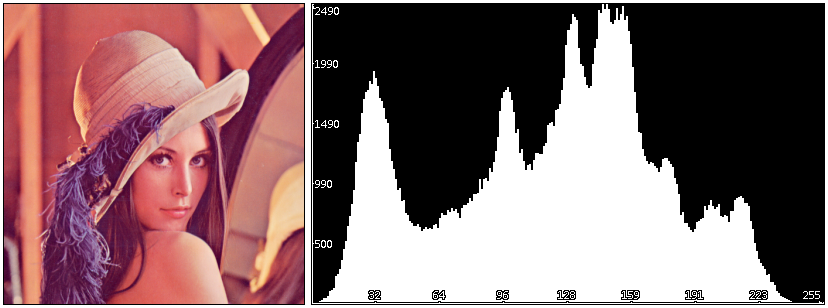
\includegraphics[width=11cm]{Bilder/histogram} \\
 \caption{Histogramm über die Helligkeitswerte eines Bildes}
 \source{http://opensource.graphics/tag/histogram/}{13.3.2019}
 \label{fig:Histogramm}
\end{figure}

Anhand des Histogramms lässt sich beispielsweise der Kontrast eines Bildes ersehen. 
Dieser beschreibt die Spannweite zwischen dem dunkelsten und dem hellsten Punktes in einem Bild, bzw. der Klassen in einem Histogramm.
Dadurch lässt sich auch der Kontrast erhöhen, indem eine Spreizung des Histogramms durchgeführt wird: Der Wertebereich der belegten Grauwertklassen wird auf den gesamten Farbbereich abgebildet 

\section{Faltungskerne} % Mo
\label{sec:Faltungskerne}
Faltungskerne beschreiben Filter in der Bildverarbeitung, die über die diskrete Faltung im 2-dimensionalen
Raum auf ein Bild angewendet werden.

Grundsätzlich ist die 1-dimensionale Faltung im kontinuierlichen Raum durch die Integration zweier Funktionen {\em g} und {\em f} an einem Punkt {\em t} definiert, wobei die Funktion {\em g} gespiegelt wird, also auf {\em f} gefaltet wird:

$$ (f * g)(t) = \int_{-\infty}^{\infty} f(\tau)g(t - \tau) d\tau $$

Für die Bildverarbeitung ist jedoch die Faltung im diskreten 2-dimensionalen Raum relevant.
Hierfür wird statt dem Integral, die Doppelsumme über alle Werte {\em n} gebildet (in {\em x}- und {\em y}-Richtung) und der Filter {\em k} mit dem Bild {\em I} an einem Punkt {\em (x, y)} gefaltet:

$$ I\mbox{*}(x, y) = \sum_{i=1}^{n}\sum_{j=1}^{n} I(x - i, y - j)k(i, j) $$

Hiermit wird nun eine Faltungsmatrix, bzw. ein Faltungskern auf jeden Pixel im Bild angewendet:

$$ k = \left( \begin{array}{rrr}
1 & 1 & 1 \\
1 & 1 & 1 \\
1 & 1 & 1 \\
\end{array}\right) $$

Faltungskerne sind lokale Operatoren, die die Neuberechnung eines Pixels mittels eines Teilbereichs des Bildes durchführen.
Mit solchen Filtern lassen sich Bilder beispielsweise Schärfen, Glätten. Es lassen sich jedoch auch Kanten finden oder Rauschanteile reduzieren.

\subsection{Gauß-Filter}
Der Gauß-Filter ist ein Faltungskern, der über eine gaußsche Glockenkurve gebildet wird.
Mit solch einem Filter lassen sich Bilder glätten und somit Rauschanteile reduzieren.
Bilder wirken dadurch weicher, bzw. verwaschen.

Ein möglicher Faltungskern sähe so aus:

$$ \frac{1}{16} \left( \begin{array}{rrr}
1 & 2 & 1 \\
2 & 4 & 2 \\
1 & 2 & 1 \\
\end{array}\right) $$

Wendet man diesen Filter auf ein Bild mit der diskreten Faltung an, erhält man dieses Ergebnis:

\begin{figure}[ht]
   \centering
     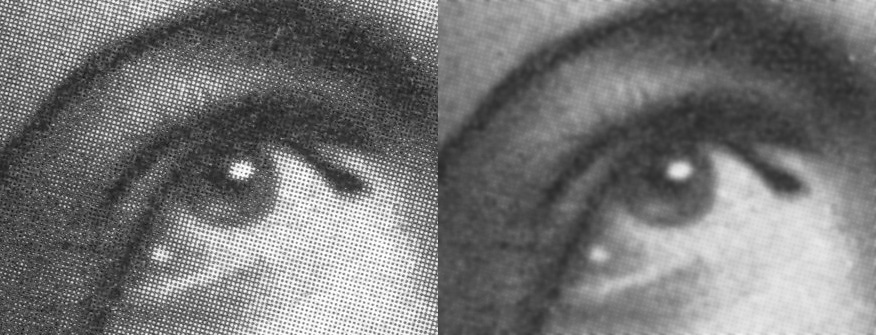
\includegraphics[width=11cm]{Bilder/Gaussian_Blur} \\
 \caption{Anwendung eines Weichzeichnungsfilters}
 \source{https://de.wikipedia.org/wiki/Datei:Halftone,_Gaussian_Blur.jpg}{10.3.2019}
 \label{fig:Blur}
\end{figure}

\subsection{Laplace-Filter}
Ein Laplace-Filter ist ein Faltungskern zur Kantendetektion innerhalb eines Bildes.
Unter einer Kante versteht man eine rasche Veränderung der Helligkeitswerte entlang einer Richtung.

Um Kanten zu finden wird ein Operator auf das Bild angewendet, der die zweite Ableitung bildet (Laplace-Operator). Abrupte Schwankungen der Intensitätswerte werden dadurch als Nulldurchgänge sichtbar.

Über die Faltung des Operators der Vorwärtsdifferenz {\em (1 -1)} mit sich selbst, lässt sich ein 1-dimensionaler Faltungskern der zweiten Ableitung bilden: {\em (1 -2 1)}.
Dieser Kern lässt sich transponieren, um ein Bild nicht nur in x-, sondern auch in y-Richtung abzuleiten.
Beide Kerne kombiniert ergeben den Laplace-Filter:

$$ \left( \begin{array}{rrr}
0 & 1 & 0 \\
1 & -4 & 1 \\
0 & 1 & 0 \\
\end{array}\right) $$

Wendet man diesen Filter auf ein Bild an, erhält man folgendes Ergebnis:

\begin{figure}[ht]
   \centering
     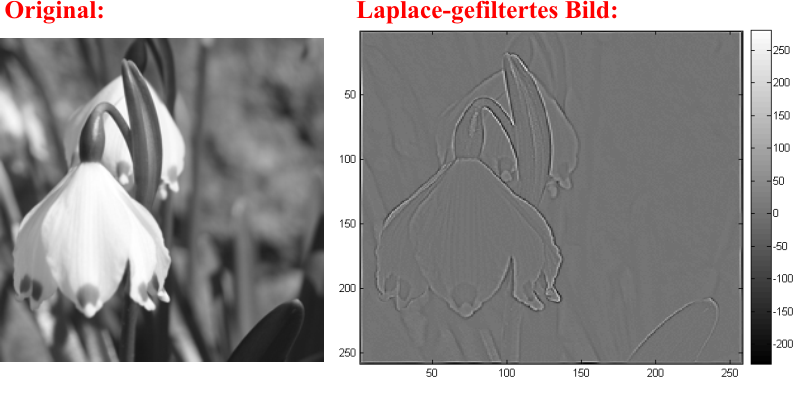
\includegraphics[width=11cm]{Bilder/Laplace} \\
 \caption{Anwendung eines Laplace-Filters}
 \source{https://de.wikipedia.org/wiki/Datei:Laplace_beispiel.png}{10.3.2019}
 \label{fig:Laplace}
\end{figure}

Aufgrund eines hohen Rauschanteils in natürlichen Bildern liefert dieser Filter jedoch nicht immer gute Resultate.

\subsection{Sobel-Operator}
\label{sec:Sobel}
Um auf natürlichen Bildern Kanten zuverlässig zu erkennen, kombiniert der Sobel-Operator die Ideen des Gauß- und Laplace-Filters.
Das Bild wird in eine Richtung über die zentrale Differenz {\em (1 0 -1)} abgeleitet, in die andere Richtung jedoch über einen Gauß-Filter {\em (1 2 1)} geglättet,
um Rauschanteile zu reduzieren.
Kombiniert man beide Filter miteinander, erhält man den Sobel-Operator.

$$ \left( \begin{array}{rrr}
-1 & 0 & 1 \\
-2 & 0 & 2 \\
-1 & 0 & 1 \\
\end{array}\right) $$

Dadurch werden Kanten jedoch nur in eine Richtung erkannt.
Um Kanten in die jeweils andere Richtung zu erkennen, kann die Faltungsmatrix transponiert werden und ebenfalls auf
das Ausgangsbild angewendet werden.

Die beiden erhaltenen Ergebnisse können nun vereint werden, um alle Kanten innerhalb eines Bildes zu erhalten:

\begin{figure}[ht]
   \centering
     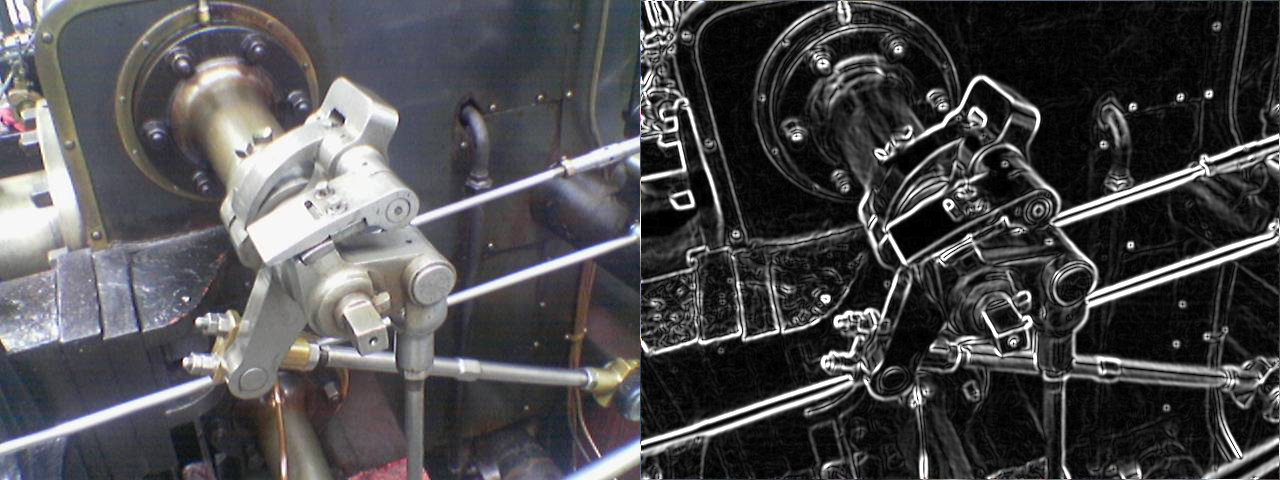
\includegraphics[width=11cm]{Bilder/Sobel} \\
 \caption{Anwendung eines Sobel-Operators}
 \source{https://en.wikipedia.org/wiki/File:Valve_sobel_(3).PNG}{10.3.2019}
 \label{fig:Sobel}
\end{figure}

%\section{Canny-Edge-Detection} % Mi
% Vlt. raus?

\section{Otsu} % Mi
Das Verfahren von Otsu dient zur Bildsegmentierung.
Durch die Findung eines geeigneten Schwellwertes, sollen Grauwerte eines Bildes über das Histogramm in zwei Klassen eingeteilt werden.
Die beiden Klassen werden so gewählt, dass die Varianz der Grauwerte innerhalb der Klassen möglichst gering ist, jedoch zwischen den Klassen möglichst groß.

Der Grauwert, der beide Klassen voneinander trennt, ist gleichzeitig der Schwellwert zur Segmentierung des Bildes. Ist der Grauwert eines Pixels unter dem Schwellwert, gehört er zur 1. Klasse, ansonsten zur 2. Klasse.
Abhängig davon wie das Bild geartet ist, lässt sich eine Klasse als Hintergrund interpretieren und die jeweils andere beschreibt den Vordergrund, bzw. das gewünschte Objekt.

\begin{figure}[ht]
   \centering
     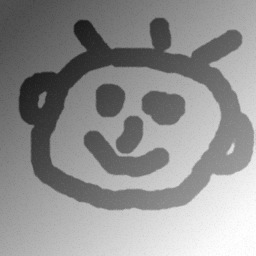
\includegraphics[width=4cm]{Bilder/otsu-1}
     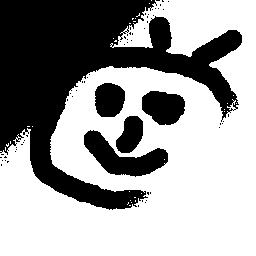
\includegraphics[width=4cm]{Bilder/otsu-2} \\
 \caption{Segmentierung eines Bildes mit dem Otsu Verfahren}
 \source{https://de.wikipedia.org/wiki/Schwellenwertverfahren\#Verfahren_von_Otsu}{29.3.2019}
 \label{fig:Otsu}
\end{figure}

Dadurch, dass ein globaler Schwellwert für das gesamte Bild verwendet wird, haben globale Helligkeitseinflüsse wie Licht und Schatten starke Auswirkungen auf das Ergebnis des Verfahrens, wie in Abbildung~\ref{fig:Otsu} zu erkennen ist. Um solche Störfaktoren zu umgehen, kann, statt eines globalen Schwellwertes auch ein lokaler Schwellwert für jeden Pixel anhand seiner Nachbarschaft individuell bestimmt werden. So kommt es unter Umständen u genaueren Ergebnissen.
Für weitere Literatur, siehe~\cite{Otsu}.

\section{Haar Kaskaden} % Mi
Mittels Haar Kaskaden lassen sich relativ schnell Objekte innerhalb eines Bildes identifizieren.

Die Grundlage hierfür bilden {\em Haar Features}~\ref{fig:Haar}.
Das sind Features, die einen Pixelverlauf als Kante, Linie oder Rechteck einstufen.

\begin{figure}[ht]
   \centering
     
\includegraphics[width=11cm]{Bilder/Haar} \\
 \caption{Haar Features}
 \source{https://commons.wikimedia.org/wiki/File:VJ_featureTypes.svg}{30.3.2019}
 \label{fig:Haar}
\end{figure}

Diese können ebenfalls als Faltungsmatrix dargestellt werden.
Eine bestimmte Menge und Kombination dieser Features beschreibt anschließend das gesuchte Objekt.
Sie müssen jedoch im Bild zuerst erkannt werden, was selbst bei einer geringen Auflösung sehr aufwendig werden kann.

Da diese Features auch nur einen geringen Teil des Bildes ausmachen, wird die Erkennung dieser in eine Kaskade unterteilt: Das Bild wird zunächst grob nach den Features durchsucht, und anschließend in den Bereichen die Suche verfeinert, in denen die gewünschten Features vorkommen könnten, sodass eine Kaskade von Suchen durchlaufen wird, bis die Features entweder gefunden oder nicht gefunden wurden und das Bild entsprechend eingestuft werden kann.
Für weitere Informationen, siehe~\cite{haar}.

\section{Morphologische Operatoren} % Mo
\label{sec:MorphologischeOperatoren}
Morphologische Operatoren werden in der Bildverarbeitung eingesetzt, um die Form von Strukturen innerhalb eines Bildes zu verändern.
Sie können sowohl auf Binär-, als auch auf Grauwertbildern angewendet werden, wobei hier lediglich auf die Anwendung bei Binärbildern
eingegangen wird.

Zunächst gibt es einfache Basisoperationen, wie Erosion und Dilatation, die die Basis für weitere, komplexere morphologische Operatoren, wie beispielsweise Opening und Closing, bilden.

\subsection{Erosion}
Bei der Erosion werden Strukturen, wie der Name vermuten lässt, erodiert bzw. abgetragen.
Man definiert hierfür eine Maske, üblicherweise ein Raster von 3x3 Pixeln, wobei der Kern der Maske auch der Mittelpunkt des Rasters ist.

Für jeden gesetzten Pixel (mit Wert 1) innerhalb des Binärbilds wird nun die Maske aufgelegt. Sind dabei nicht alle anderen Pixel innerhalb der Maske ebenfalls gesetzt, so wird das Pixel im resultierenden Bild auf den Wert 0 gesetzt.
Haben jedoch alle Nachbarn eines Pixels innerhalb der Maske ebenfalls den Wert 1, so verändert sich das Pixel nicht.

Formal wird die Erosion folgendermaßen notiert: $ I \ominus M $. Wobei das Bild {\em I} mit der Maske {\em M} erodiert wird.

Der daraus resultierende Effekt ist, wie in Abbildung~\ref{fig:Erosion} ersichtlich, dass Ränder von Strukturen innerhalb des Bildes abgetragen werden und diese somit verdünnt werden. Es können aber auch Löcher innerhalb der Strukturen vergrößert werden.

\begin{figure}[ht]
   \centering
     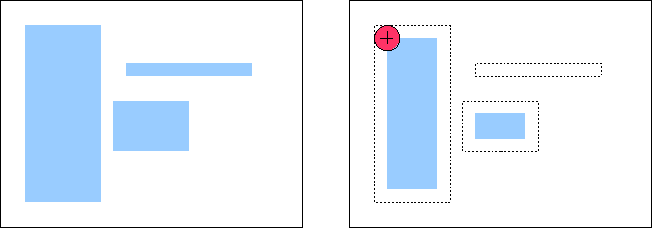
\includegraphics[width=11cm]{Bilder/MorphologicalErosion} \\
 \caption{Anwendung der Erosion auf ein Bild}
 \source{https://de.wikipedia.org/wiki/Datei:MorphologicalErosion.png}{12.3.2019}
 \label{fig:Erosion}
\end{figure}

\subsection{Dilatation}
Die Dilatation bildet das Gegenstück zur Erosion. Statt die jeweiligen Strukturen abzutragen, lässt man diese wachsen.
Dabei kann dieselbe Maske wie bei der Erosion verwendet werden. Diese muss ebenfalls für jeden Pixel auf das Binärbild aufgelegt werden. Ist der Kern der Maske, also das Pixel auf welches die Maske gelegt wurde gesetzt, so werden im resultierenden Bild alle Pixel innerhalb der Maske ebenfalls gesetzt. Hat der Kern jedoch den
Wert 0, so verändert sich für dieses Pixel nichts.

Die formale Notation ist $ I \oplus M $, wobei hier Bild {\em I} mit Maske {\em M} dilatiert wird.

Wie in Abbildung~\ref{fig:Dilation} erkennbar, wachsen die Strukturen innerhalb des Bildes. Dabei können vorher getrennte Strukturen zusammenwachsen oder Löcher innerhalb einer Struktur geschlossen werden.

\begin{figure}[ht]
   \centering
     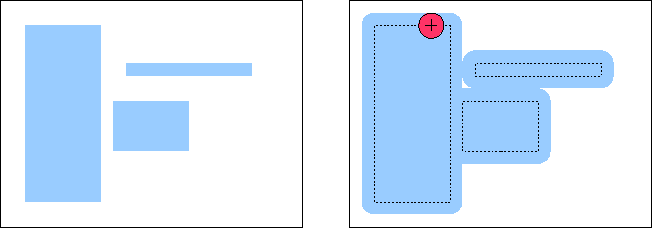
\includegraphics[width=11cm]{Bilder/MorphologicalDilation} \\
 \caption{Anwendung der Dilatation auf ein Bild}
 \source{https://de.wikipedia.org/wiki/Datei:MorphologicalDilation.png}{12.3.2019}
 \label{fig:Dilation}
\end{figure}

\subsection{Opening}
Im Gegensatz zu den vorhergehenden Operationen ist das Opening keine Basisoperation mehr, sondern setzt sich aus den Basisoperationen zusammen.
Dabei wird ein Bild {\em I} zunächst mit einer Maske {\em M} erodiert und anschließend dilatiert:

$$ I \circ M = ( I \ominus M ) \oplus M $$

Die Struktur von hinreichend großen Elementen wird durch diese Operation nicht verändert. Es werden lediglich kleinere Artefakte, welche zumeist durch Störungen oder Rauschen innerhalb des Ursprungsbildes entstanden sind, durch Erosion entfernt. Durch die anschließende Dilatation können diese nicht mehr erzeugt werden. Es können auch Strukturen, die über eine Verbindungsstelle, welche schmäler als die Maske ist, voneinander getrennt werden, sodass aus einer Struktur zwei getrennte entstehen.
Ein Beispiel lässt sich in Abbildung~\ref{fig:Opening} sehen.

\begin{figure}[ht]
   \centering
     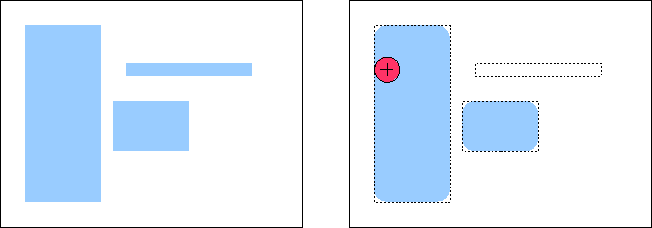
\includegraphics[width=11cm]{Bilder/MorphologicalOpening} \\
 \caption{Anwendung von Opening auf ein Bild}
 \source{https://de.wikipedia.org/wiki/Datei:MorphologicalOpening.png}{12.3.2019}
 \label{fig:Opening}
\end{figure}

\subsection{Closing}
Closing bildet das Gegenstück zu Opening.
Ein Bild {\em I} wird mit einer Maske {\em M} dilatiert und anschließend erodiert:

$$ I \bullet M = ( I \oplus M ) \ominus M $$

Genutzt werden kann dieser Operator, um beispielsweise, wie der Name erschließen lässt, Löcher in Strukturen zu schließen, oder Verbindungen zwischen vorher getrennten Strukturen aufzubauen.
Durch die Dilatation werden Lücken geschlossen, bzw. nahe beieinander liegende Strukturen verbunden. Die Größe der Elemente wird durch die anschließende Erosion wieder zurückgesetzt. Entstandene Verbindungen und geschlossene Lücken bleiben dadurch jedoch erhalten.
Ein Beispiel ist in Abbildung~\ref{fig:Closing} zu sehen.

\begin{figure}[ht]
   \centering
     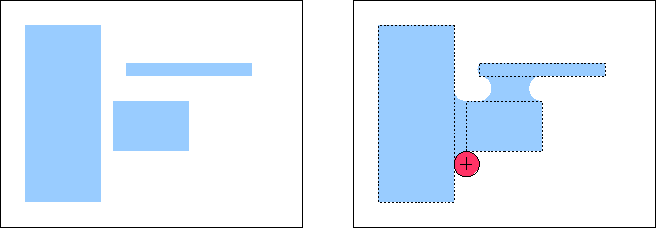
\includegraphics[width=11cm]{Bilder/MorphologicalClosing} \\
 \caption{Anwendung von Closing auf ein Bild}
 \source{https://de.wikipedia.org/wiki/Datei:MorphologicalClosing.png}{12.3.2019}
 \label{fig:Closing}
\end{figure}

\section{OpenCV} % Mi
\label{sec:OpenCV}
OpenCV ist eine Programmierbibliothek, die eine Reihe von Bildverarbeitungsalgorithmen zur Verfügung stellt.
Es gibt Implementierungen in C, C++, Java und einigen weiteren Programmiersprachen. Unter anderem gibt es auch eine Bibliothek für Android Geräte.

Es existieren diverse Hilfsmittel zur Segmentierung und Klassifikation von Bildern. Darüber hinaus werden auch morphologische Operatoren bereitgestellt. Durch die Kombination verschiedener Algorithmen und Hilfsmittel hat man als Programmierer die Möglichkeit, sich eine Bildverarbeitungspipeline aufzubauen, um seine Bilder zu verarbeiten. Für mehr Informationen, siehe~\cite{opencv}.
